\section{Validation Results}
\label{sec:ValidationResults}

\subsection{Trade off Aperture and Power}
\label{sec:PowerApertureTradeoff}

In order to correctly determine the lasing power and the sizing of the receiver aperture, an optimization problem was created. This problem describes how the sizing of both the laser and receiver relate to the total amount of received photons. The method used to solve this problem is the Nelder-Mead (or downhill simplex) method as implemented is the Apache Commons Math library.

The most important parameter is the target amount of photons per pulse per satellite. This reflects the quality of the data. The target is set to 10 photons detected per transmitted pulse, as this will guarantee a decent quality in the \ac{BRDF} reconstruction. As initial parameters, a power of 5 W and an aperture of $10\times10$ cm are used. The performance of each iteration is quantified using equation \ref{eq:PowerAperturePerformance}:

\begin{equation}
	\text{perf} = \frac {f(\varphi_{total}, \varphi_{target} \times \text{\# sats}, 50) \times 
												\displaystyle\prod_{sat} f(\varphi_{sat}, \varphi_{target}, 200) }
											{ \text{power} \times \text{aperture}^{1.2}}
	\label{eq:PowerAperturePerformance}
\end{equation}

In this equation, $f(x, mean, variance)$ is a normal distribution given mean and variance evaluated at x. A visualization of the results can be seen in figure \ref{fig:PowerAperturePerformance}. It shows the region around the local maximum for the performance function. To summarize, the results of the optimization algorithm are:

\begin{itemize}
	\item Power 4.6 W
	\item Aperture 0.0045 m$^2$ (or $6.7\times6.7$ cm)
\end{itemize}

\begin{figure}[ht]
	\centering
	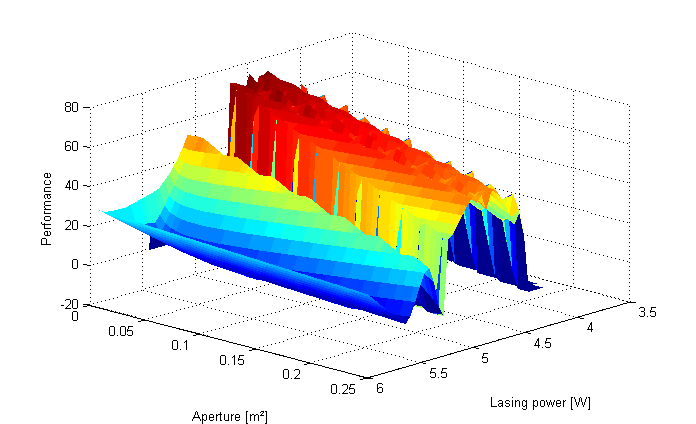
\includegraphics[width=0.6\textwidth]{chapters/img/optimize-PowerAperture.png}%
		\caption{Power-Aperture optimization visualization}%
		\label{fig:PowerAperturePerformance}%
\end{figure}

Note, these results are the bare minimum for the system to operate as designed. When taking a safe margin, this translates into a minimal lasing power of 5.5 W and an aperture of 0.0055 m$^2$ ($7.5\times7.5$ cm). 

\subsection{Height Reconstruction}
\label{sec:HeightReconstruction}

The height reconstruction algorithm takes as an input the photons received by the various satellites and the times they were received. Then the photon stream is divided in \emph{interpulse windows}. And interpulse window is as long as one over the pulse frequency. To cut down data volume, the photons inside an interpulse window are divided into a signal window and a noise window. The signal window is centered around the time the signal ought be received (as reconstructed from the emitter history) and bounded by the minimum land elevation ($\sim -500\ m$, for the Dead Sea) and the maximum land elevation (Mt. Everest, $\sim 9000\ m$); any photon that would render another height is not possible on the Earth, and can be discarded directly.

The signal photons are still a pretty mixed lot of noise and actual laser photons, and the next step is to separate the data from the noise. This is done by putting the photons in associated groupings. Before grouping, though, every photon is converted to a height. This is done by constructing an ellipse with the emitter and receiver satellites at the foci, and by setting the angles correctly (from the nadir-pointing requirements) the height is reconstructed.

Then the heights obtained are grouped based on the difference between the altitudes. So for example, if one altitude is found for 50 meters, and the second one is for 50.2 meters, they are recognized as representing the same elevation and grouped together. After the grouping is done, the largest grouping is picked and averaged, and that is the height that is eventually selected. Because the laser photons are much, much more concentrated than the noise photons are, this will filter out the noise and leave us with the data photons; this generally gives a pretty good estimate of the height along the groundtrack.

To improve output quality, further post-processing takes place. The first type of filter used is \emph{spike filtering}. In spike filtering, a data point and the two adjacent heights are compared; if the middle one is more than a certain offset off, it is replaced by the average of the two adjacent points. Another algorithm is \emph{averaging outlier detection}. In this algorithm, a running average is kept, and if the datapoint diverges too much from the average, it is substituted by the average.

When an altitude is substituted, either by the spike or the averaging outlier detection filtering, the program goes through the altitude groupings and looks for the one closest to the average, takes that grouping, averages it and substitutes it for the old value. This means that the filters are smarter than they look: they do not just pull data out of the air, but they actually reconsider the signal photons available. This makes the filtering very robust.

For the height determination, accuracies of 3 cm can be obtained when not taking into account sloping, which is as large as the precision caused by the maximum time uncertainty of 97 picoseconds, meaning that, without sloping, the algorithm is perfectly accurate at determining the original height distribution. When sloping is applied to the terrain, accuracy dimishes somewhat, especially over heavily sloping or topographically varying terrain. Because the bandwidth over which the data photons are spread out increases, the chances of noise photons being included increase. This in turn causes more variation in the signal, and standard deviations for moderately sloped terrain are in the range of ten to a few tens of centimeters. This does vary a lot for topographically more extremely varying results though. How this affects data validity will have to be researched in a further study.

Note that, even for extremely sloped terrain, a measurement taken by night will have a 3 cm accuracy, due to the absense of thermal and solar noise. So if for a certain terrain it would be too sloped for daylight measurement, night time measurements will still give accurate terrain information. This is, however, a last resort. If it is needed will need to be determined by further studies.

\subsection{Slope}
\label{sec:Slope}
To facilitate \ac{BRDF} reconstruction, the slopes are calculated. The along track slope is simply found by averaging the slope over the last few datapoints. The cross track slope is a little more difficult. Two approaches can be taken. 

The first option is to determine the total slope within the footprint based on the height variation within the footprint, found from the different data photons. Now the slope is rotated so as to match the along track slope, and then the cross track slope is set so that, when added to the along track slope, it renders the total slope in the footprint. Whereas this sounds nice in theory, the practice is a lot harder, because the horizontal spread of the different subfootprint points is unknown, and has to be assumed. This assumption introduces a rather large error into the cross track slope.

A second and simpler way is to take the subdivision of the footprint as caused by the effect of having 9 to 16 detectors pointing at the footprint. This means that cross track slope determination can easily done, because the horizontal distance between the ground points is approximately known. However, the simulator was well under way to being written before the 32 by 32 \ac{SPAD} array was found and chosen as a receiver instrument. This means that the multiple detectors are not implemented in the code yet, and implementing them in the code would need to be done by a further development of the code.

It is clear that the along track slope can be calculated with greater accuracy and confidence then the cross track slope.

\subsection{\ac{BRDF} Reconstruction}
\label{sec:BRDFReconstuction}

To exploit the multi-angular observation and to demonstrate extra functionality of the Laser Swarm an attempt is made to determine the \ac{BRDF}. 
The \ac{BRDF} is useful in determining the anisotropic reflectance properties of the surfaces on the ground that way aiding elimination of the noise. Furthermore the \ac{BRDF} can be used to determine the Vegetation Index (VI) by correlating the \ac{BRDF} with other geomatic data \cite{BRDFwanner}. The \ac{BRDF} could also be used to determine such things as the amount of foam, oil or algae on water bodies.

In reality, the height distribution within a footprint is responsible for effects such as shadowing, masking and re-reflections \cite{BRDFsparrow}. A footprint also can be comprised of different materials therefore having a varying \ac{BRDF}. In the scientific community a model was established to model the \ac{BRDF} for a flat surface, in theory this model could be extended to model the \ac{BRDF} of a footprint as a function of the height distribution, however, this is outside the scope of this feasibility study. 

Multiple footprints are necessary to more accurately determine the \ac{BRDF}. Thankfully, for every part of the terrain there are 45 overlapping measurements, so this is not a problem. Using this oversampling, the concept of region is defined. Each region consists of multiple footprints, and for each region the \ac{BRDF} is calculated.

To measure the \ac{BRDF}, all that is needed is the normal vector of the plane illuminated by the footprint and the amount of the received photons in the specific direction. As the slope of the local plane and the position of the receivers change (with the constellation progressing along the orbit), photons are registered from a different point of view for every footprint. The number of received photons in a specific direction with respect to the total amount of photons corresponds to the relative magnitude of the \ac{BRDF} in that direction. Since the maximum inclination of the receiver with respect to the normal is $30^\circ$ only a small cone of the \ac{BRDF} is obtained. Furthermore, the amount of points registered per footprint is at most the amount of receivers in the swarm, and since the observed region on the ground changes much faster than the change in relative position of the receiver satellites, the registered points are not spread out through out the whole \ac{BRDF} sphere but are confined to a small region. 

For practical purposes \ac{BRDF} does not need to be known exactly, so to make the inversion process easier various semi-empirical models of \ac{BRDF} exist. Semi-empirical models approximate the shape of the \ac{BRDF} by means of some a-priori information \cite{BRDFwanner}. So in order to invert \ac{BRDF} from measured points, coefficients in the following equation need to be found:

\[
R(\theta ,\vartheta ,\phi ) = f_{iso}  + f_{geo} K_{geo} (\theta ,\vartheta ,\phi ) + f_{vol} K_{vol} (\theta ,\vartheta ,\phi )
\]


with $R$ representing relative radiance as a function of the position of the light source ($\theta$) and position of the observer ($\vartheta$, $\phi$), and $f_{iso}$  , $f_{geo}$, $f_{vol}$  being the coefficients that need to be determined. $K_{geo}$ and $K_{vol}$ are so called kernels which are functions of the incident light and they are known in advance. Different types of kernels exist, each of them suited better for different types of terrain under consideration. 
For the purpose of simulation a simplified empirical model will be used:

\[
R_{{\rm{model}}} (\theta ,\vartheta ,\phi ){\rm{ }} = {\rm{ }}p_0 (\theta _{}^2  + \vartheta _{}^2 ) + p_1 \vartheta _{}^2 \theta _{}^2  + p_2 \vartheta \theta \cos (\phi ) + p_3 
\]

The coefficients $p_0$, $p_1$,$p_2$,$p_3$ are estimated from measured data by means of multivariable regression analysis \cite{BRDFrob}. 

The \ac{BRDF} calculation algorithm does not take into account the height distribution within the footprint and assumes that the \ac{BRDF} within the footprint remains the same. These assumptions are valid as the height distribution within the footprint and the \ac{BRDF} are indistinguishable from each other. However as the overall height distribution is random, that roughly corresponds to Lambergian \ac{BRDF} and can be treated as a systematic error that can affects all results equally. The assumption that the \ac{BRDF} is constant within the footprint is supported by the fact that in the observation missions the area being measured is usually multiple orders of magnitude larger than the footprint.



